\normalfont\documentclass[letterpaper,11pt]{article}
\usepackage{amsmath, amsfonts,amssymb,latexsym}
\usepackage{fullpage}
\usepackage{parskip}
\usepackage{graphicx}

\begin{document}

\newcommand{\header}{
	\noindent \fbox{
	\begin{minipage}{6.4in}
  	\medskip
  	\textbf{ACM algorithm practice} \hfill \textbf{Fall 2015} \\[1mm]
  	\begin{center}
    	{\Large Week 1 Problems} \\[3mm]
  	\end{center}
	\today \hfill \itshape{Timothy Johnson}
	\medskip
	\end{minipage}}
}

\bigskip
%\header

\section*{Problem 1: Run for beer}
People in BubbleLand like to drink beer. Little do they know, beer here is so good and strong that every time they drink it their speed is 10 times slower than before they drank it.

Birko lives in the city Beergrade, but wants to go to the city Beerburg. You are given a road map of BubbleLand and you need to find the fastest way for him. When he starts his journey in Beergrade his speed is 1. When he comes to a new city he always tries a glass of local beer, which divides his speed by 10.

The question here is what the minimal time is for him to reach Beerburg. If there are several paths with the same minimal time, pick the one that has fewest roads on it. If there is still more than one path, pick any.

It is guaranteed that there will be at least one path from Beergrade to Beerburg.

\textbf{Input} \newline
The first line of input contains an integer $N$, the number of cities in Bubbleland, and an integer $M$, the number of roads in this country. Cities are enumerated from 0 to $N - 1$, with city 0 being Beergrade, and city $N - 1$ being Beerburg. Each of the following $M$ lines contains three integers $a, b, len$, where $a \neq b$. These numbers indicate that there is a bidirectional road between cities $a$ and $b$ with length $len$.

The problem sizes are: $2 \leq N \leq 10^5$, $1 \leq M \leq 10^5$, $0 \leq len \leq 9$. There is at most one road joining any two cities.

\textbf{Output} \newline
The first line of output should contain the minimal time neeed to go from Beergrade to Beerburg. The second line should contain the number of cities on this shortest path. The final line should contain the numbers of the cities on this path in the order they are visited, separated by spaces.

\textbf{Examples}
\begin{itemize}
\item \textbf{Input} \newline
8 10 \newline
0 1 1 \newline
1 2 5 \newline
2 7 6 \newline
0 3 2 \newline
3 7 3 \newline
0 4 0 \newline
4 5 0 \newline
5 7 2 \newline
0 6 0 \newline
6 7 7

\textbf{Output} \newline
32 \newline
3 \newline
0 3 7
\end{itemize}

\newpage


\section*{Problem 2:}
(Taken from: https://projecteuler.net/problem=250) \newline

Find the number of non-empty subsets of $\{1^1, 2^2, 3^3, \ldots, 250250^{250250}\}$, the sum of whose elements is divisible by 250. Enter the rightmost 16 digits as your answer.



\section*{Problem 3: Crack-Free Walls}
(Taken from: https://projecteuler.net/problem=215) \newline
Consider the problem of building a wall out of $2 \times 1$ and $3 \times 1$ bricks (horizontal and vertical dimensions) such that, for extra strength, the gaps between horizontally-adjacent bricks never line up in consecutive layers, i.e., never form a running crack.

For example, the following $9 \times 3$ wall is not acceptable due to the running crack shown in red:

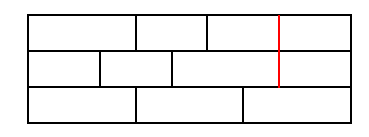
\includegraphics{PE215_fig.png}

There are eight ways of forming a crack-free $9 \times 3$ wall, written $W(9,3) = 8$.

Calculate $W(32,10)$.

Note: Project Euler problems have no enforced time limit, but there is always a solution that takes well under a minute in a reasonably fast language on a standard computer.

\end{document}